
% % \begin{algorithm}[htbp]
%     \caption{Bron-Kerbosch Algorithm}
%     \label{alg:bron_kerbosch}
%     \KwIn{Graph $G = (V, E)$}
%     \KwOut{All maximal cliques in $G$}
%     \SetKwFunction{FMain}{BronKerbosch}
%     \SetKwProg{Fn}{Function}{:}{}
%     \Fn{\FMain{$R, P, X$}}{
%         \If{$P = \emptyset \land X = \emptyset$}{
%             \Return $R$ \;
%         }
%         $u_{piv} \gets \arg\max_{x\in P} |P\cap N_H(x)|$ \;
%         \ForEach{$v \in P \setminus N(u_{piv})$}{
%             \FMain{$R \cup \{v\}, P \cap N(v), X \cap N(v)$} \;
%             $P \gets P \setminus \{v\}$ \;
%             $X \gets X \cup \{v\}$ \;
%         }
%     }
% \end{algorithm}

% \begin{algorithm}[htbp]
%     \caption{Bron-Kerbosch Algorithm}
%     \label{alg:bron_kerbosch}
%     \LinesNumbered
%     \KwIn{Undirected graph $G=(V,E)$}
%     \KwOut{All maximal cliques in $G$}
%     \SetKwFunction{BKMain}{BronKerbosch}
%     \SetKwProg{Fn}{Function}{:}{}

%     Compute a degeneracy ordering $(v_1,\dots,v_n)$ of $G$; let $\sigma(v_i)\leftarrow i$\;
%     Orient every edge from lower to higher rank to obtain $N^{+}(\cdot)$;
    
%     \ForEach{$v \in V$ in increasing order of $\sigma$}{
%         $P \gets N^{+}(v)$,\quad $X \gets N(v)\setminus N^{+}(v)$\;
%         \BKMain{$\{v\},\; P,\; X$}\;
%     }

%     \Fn{\BKMain{$R, P, X$}}{
%         \If{$P=\emptyset \land X=\emptyset$}{
%             \textbf{output clique }$R$\;
%             \Return
%         }
%         $u_{\text{piv}} \gets \arg\max_{x \in P \cup X} |\,P \cap N(x)\,|$ 
        
%         \ForEach{$v \in P \setminus N(u_{\text{piv}})$}{
%             \BKMain{$R \cup \{v\},\; P \cap N(v),\; X \cap N(v)$}\;
%             $P \gets P \setminus \{v\}$\;
%             $X \gets X \cup \{v\}$\;
%         }
%     }
    
    
% \end{algorithm}

% \begin{algorithm}[htbp]
%     \caption{Bron-Kerbosch Algorithm}
%     \label{alg:bron_kerbosch}
%     \KwIn{Graph $G=(V,E)$}
%     \KwOut{All maximal cliques in $G$ (each reported once)}
%     \SetKwFunction{BKMain}{BronKerbosch}
%     \SetKwProg{Fn}{Function}{:}{}

%     Compute a degeneracy ordering $(v_1,\dots,v_n)$ of $G$  
%     Orient every edge from lower to higher rank to obtain $N^{+}(\cdot)$\;

%     \ForEach{$v \in V$ in increasing order of $\sigma$}{
%         $P \gets N^{+}(v)$\;
%         \BKMain{$\{v\}, P$}\;
%     }

%     \Fn{\BKMain{$R, P$}}{
%         \If{$P=\emptyset$}{
%             \Return $R$ 
%         }
%         $u_{\text{piv}} \gets \arg\max_{x\in P} |P \cap N(x)|$ 

%         \ForEach{$v \in P \setminus N(u_{\text{piv}})$}{
%             \BKMain{$R \cup \{v\},\;\; P \cap N(v)$}\;
%             $P \gets P \setminus \{v\}$ 
%         }
%     }
    
% \end{algorithm}




% \begin{algorithm}[t!]
%     \caption{\textsc{Build--SCT}$(G,\,s)$}
%     \label{alg:buildSCT}
%     \KwIn{Undirected graph $G=(V,E)$, optional size cap $s$}
%     \KwOut{Succinct Clique Tree of $G$}

%     Compute a degeneracy ordering $(v_1,\dots,v_n)$ of $G$  
%     Orient every edge from lower to higher rank to obtain $N^{+}(\cdot)$\;

%     \For(\tcp*[f]{one root per vertex}){$i\gets 1$ \KwTo $n$}{
%         $V_{Hold}\gets\{v_i\}$ $P\gets N^{+}(v_i)$ $V_{Pivot}\gets\emptyset$

%         \textsc{ExpandPath}$(P, V_{Hold}, V_{Pivot})$\;
%     }

%     \SetKwFunction{Expand}{ExpandPath}
%     \SetKwProg{Fn}{Function}{:}{}

%     \Fn{\Expand{$P, V_{Hold}, V_{Pivot}$}}{
%         \If{$P=\emptyset$}{
%             \textbf{output path }$\{V_{Hold},\,V_{Pivot}\}$\;
%             \textbf{return}
%         }
        
%         $u_{piv} \gets \arg\max_{x\in P} |P\cap N^+(x)|$ \;
%         \For(\tcp*[f]{non-neighbors of pivot}){$v\in P\setminus N(u_{piv})$}{
%             $P\gets P\setminus\{v\}$
            
%             \eIf{$v=u_{piv}$}{
%                 \Expand{$P\cap N(v),\;V_{Hold},\;V_{Pivot}\cup\{v\}$}
%             }{
%                 \Expand{$P\cap N(v),\;V_{Hold}\cup\{v\},\;V_{Pivot}$}
%             }
%         }
%     }
% \end{algorithm}

% Lemma 4.6 (Path pruning). Let P be a path in the CPI and let
% 𝑠 ≥ 1 be the target clique size. Then P encodes at least one 𝑠-clique iff
% |𝑉ℎ (P)| ≤ 𝑠 ≤ |𝑉ℎ (P)| + |𝑉𝑝 (P)| .
% Equivalently, P can be safely pruned for size 𝑠 iff
% 𝑠 < |𝑉ℎ (P)| or 𝑠 > |𝑉ℎ (P)| + |𝑉𝑝 (P)| .
% Example 4.7. Considering the CPI shown in Figure 3, if we need

\begin{algorithm}[t!]
    \caption{\textsc{Build--CPI}$(G,\,s)$}
    \label{alg:buildCPI}
    \KwIn{Undirected graph $G=(V,E)$, optional size cap $s$}
    \KwOut{Clique Path Index (CPI) of $G$}

    Compute a degeneracy ordering $(v_1,\dots,v_n)$ of $G$  
    Orient every edge from lower to higher rank to obtain $N^{+}(\cdot)$\;

    \For(\tcp*[f]{one root per vertex}){$i\gets 1$ \KwTo $n$}{
        $V_{Hold}\gets\{v_i\}$ $P\gets N^{+}(v_i)$ $V_{Pivot}\gets\emptyset$

        \textsc{ExpandPath}$(P, V_{Hold}, V_{Pivot})$\;
    }

    \SetKwFunction{Expand}{ExpandPath}
    \SetKwProg{Fn}{Function}{:}{}

    \Fn{\Expand{$P, V_{Hold}, V_{Pivot}$}}{

    % path pruning
        \lIf{$|V_{Hold}| > s$}{
            \textbf{return}
        }

        \If{$P=\emptyset$}{
            %  \textbf{or} $|V_{Hold}| + |V_{Pivot}| < s
            % \textbf{output path }$\{V_{Hold},\,V_{Pivot}\}$\;
            % \textbf{return}
            \If{$|V_{Hold}| + |V_{Pivot}| \ge s$}{
                \textbf{output path }$\{V_{Hold},\,V_{Pivot}\}$\;
            }
            \textbf{return}
        }
        
        $u_{piv} \gets \arg\max_{x\in P} |P\cap N^+(x)|$ \;
        \For(\tcp*[f]{non-neighbors of pivot}){$v\in P\setminus N(u_{piv})$}{
            $P\gets P\setminus\{v\}$
            
            \eIf{$v=u_{piv}$}{
                \Expand{$P\cap N(v),\;V_{Hold},\;V_{Pivot}\cup\{v\}$}
            }{
                \Expand{$P\cap N(v),\;V_{Hold}\cup\{v\},\;V_{Pivot}$}
            }
        }
    }
\end{algorithm}

\subsection{Succinct Clique Tree} \label{sec:sct}

% \noindent\textit{Motivation from our base framework.}
% In the base framework (Algorithm~\ref{alg:hierarchy}, CND), three operations require an index that avoids materializing $K_s$: the one-shot initialization of $(r,s)$-supports (line 2), the path-local removal of peeled $r$-cliques (line 11), and the incremental update of neighbors' supports (line 13). Since the final output does not need to list any $s$-clique, we seek a counting representation rather than an enumeration of $K_s$.

% \noindent Succinct Clique Tree (SCT)\cite{Pivoter} is a Bron-Kerbosch-inspired representation that organizes the pivoting search space for exact clique counting.
% 
% \textit{Construction and stored semantics.} Using% \begin{definition}[clique path]
% \label{def:root_leaf_path}
% Given a \emph{Succinct Clique Tree}, a \emph{clique path}
% is a path that starts from the root node and ends at a leaf node, denoted as $\TPath{}$.
% All clique paths are enumerated in a \textbf{left-to-right
% depth-first search (DFS) order}.  We denote the $i$-th path in this
% DFS order by $\TPath{i}$.
%
% Formally, let
% \[
%   \TPath{i} = \langle v_{a_1}, v_{a_2}, \dots, v_{a_\ell} \rangle ,
% \]
% where $v_{a_1}$ is the root, $v_{a_\ell}$ is the corresponding leaf,
% and $\ell$ is the length of the path.  The index $i$ reflects the
% position of this path in the DFS enumeration described above.
% \end{definition}
%
% \begin{example}
% \label{ex:sct_example}
% Figure~\ref{fig:sct_example} shows an example of a Succinct Clique Tree
% (SCT). $\TPath{1} = \langle v_1, v_4, v_5, v_6 \rangle$, the second path is
% $\TPath{2} = \langle v_1, v_2, v_3, v_4, v_5 \rangle$. There are eleven
% clique paths in total, and the last path is $\TPath{11} = \langle v_8, v_9 \rangle$.
% \end{example}
%
%
% \begin{lemma}[Clique Count in a Path\cite{Pivoter}]
% \label{lem:clique_count}
% Let $\TPath{}$ be a clique path in an SCT, with
% $V_{p}(\TPath{})$ and $V_{h}(\TPath{})$ denoting its pivot
% and hold vertices, respectively.
% For any $k\ge |V_{h}(\TPath{})|$, every $k$-clique represented by
% $\TPath{}$ consists of all vertices in $V_{h}(\TPath{})$ and
% exactly $k-|V_{h}(\TPath{})|$ vertices chosen from $V_{p}(\TPath{})$.
% Hence $\#\text{$k$-cliques on }\TPath{}$ is equal to $ \binom{|V_{p}(\TPath{})|}{\,k-|V_{h}(\TPath{})|\,}.$
% \end{lemma}
%
% \begin{example}
%   For SCT as shown in Figure~\ref{fig:sct_example}.
%   $V_{p}(\TPath{1}) = \{v_4, v_5\}$ and
%   $V_{h}(\TPath{1}) = \{v_1,v_6\}$. Thus, the number of $3$-cliques on $\TPath{1}$ is equal to $ \binom{2}{\,3-2\,} = 2.$ $V_{p}(\TPath{2}) = \{v_2, v_3, v_4, v_5\}$ and $V_{h}(\TPath{2}) = \{v_1\}$. Thus, the number of $3$-cliques on $\TPath{2}$ is equal to $ \binom{4}{\,3-1\,} = 6.$
% \end{example} a degeneracy ordering, we orient edges from lower to higher rank to obtain $N^+(\cdot)$. For each vertex $v$ (in order), SCT starts a root with \emph{hold} set $V_h{=}\{v\}$ and \emph{pivot} set $V_p{=}N^+(v)$ and recursively expands by pivoting: choose a pivot $u\in V_p$ (e.g., maximizing $|V_p\cap N^+(u)|$) and branch only on $V_p\setminus N(u)$ while shrinking candidates to $V_p\cap N(\cdot)$. Each state stores exactly two sets—$V_h$ (already fixed) and $V_p$ (eligible extensions); along any path, $V_h$ are mandatory and $V_p$ are selectable, so a path summarizes a family of cliques without enumerating them one by one.

% \noindent\textit{SOTA counting in brief.}
% To efficiently count cliques without explicit enumeration, we first review the state-of-the-art clique counting method, the \textit{Succinct Clique Tree (\sct)}~\cite{Pivoter}. 
% \sct compacts the Bron--Kerbosch pivoting search space for exact clique counting. Vertices are processed in degeneracy order and edges are oriented to define $N^+(\cdot)$. For each root $v$, every state stores two sets—$V_h$ (hold, already fixed) and $V_p$ (pivot, eligible extensions). Pivoting on $u\in V_p$ branches only on $V_p\setminus N(u)$ while shrinking candidates to $V_p\cap N(\cdot)$. Thus each clique path succinctly summarizes a family of cliques without enumerating them.
We first review the state-of-the-art clique counting method, the \textit{Succinct Clique Tree} (\sct)~\cite{Pivoter}. 
The \sct compacts the Bron--Kerbosch pivoting search space for exact clique counting. 
Instead of enumerating all cliques, \sct constructs a hierarchical search tree in which each node corresponds to a state in the Bron--Kerbosch maximal clique search (the pivot-based version)~\cite{BronKerbosch,bitsetClique}, thereby implicitly representing all subcliques. 
Vertices are processed in \textit{degeneracy order}, and edges are oriented to define $N^+(\cdot)$. 
For each root vertex $v$ in \sct, every state maintains two sets: $V_h$ (\hold, already fixed) and $V_p$ (\pivot, eligible extensions). 
Pivoting on $u \in V_p$ branches only on $V_p \setminus N(u)$ while restricting candidates to $V_p \cap N(\cdot)$. 
Thus, each \textit{clique} path succinctly represents a family of cliques without enumerating them explicitly. 
This structure supports aggregated counting of all subcliques (of sizes $r$, $s$, etc.), enabling exact clique counting without enumeration.


% \begin{algorithm}[t]
\small
% \caption{UpdateSupport}
% \label{alg:updateSupport}
% % $R_{min}$, $I$, $support$, $H_{\min}$)
% \KwIn{$r$-cliques $R_{min}$ removed, \sct $I$, support map $support$, min heap $H_{\min}$}
% \KwOut{Updated support map $support$ and min heap $H_{\min}$}
% \SetKwFunction{UpdateIndex}{UpdateIndex}
% \SetKwProg{Fn}{Function}{:}{}

% \ForEach{path $\TPath$ in $I$ that intersects any $rc \in R_{min}$}{
%     \ForEach{$rc covered$ by $\TPath$}{
%         old$\gets support(rc)$\;
%         recompute $support(rc)$ based on $\TPath$\;
%         \If{support(rc) changed}{
%             update $H_{\min}$ with new support value\;
%         }
%     }
% }
% \end{algorithm}

% 
% Bron-Kerbosch\cite{BronKerbosch}是枚举极大团的经典算法, 其通过对三个顶点集合$R$, $P$, $X$的递归回溯来枚举所有极大团. 其中$R$表示当前已经找到的极大团, $P$表示当前可能的顶点集合, $X$表示已经被排除的顶点集合. 该算法的时间复杂度为$O(3^{n/3})$, 其中$n$是图中顶点的个数.
% \paragraph{Bron--Kerbosch enumeration framework.}

% During each recursive call it keeps three pairwise-disjoint vertex sets, 
% $R$ denotes the current (partial) clique,
% $P$ comprises those vertices that may still be added to extend $R$,
% and $X$ collects vertices that have already been explored and must therefore be excluded.
% Given a vertex $v\in P$, the algorithm moves $v$ into $R$, updates
% $P\leftarrow P\cap N(v)$ and $X\leftarrow X\cap N(v)$, and then recurses.
% When both $P$ and $X$ become empty, $R$ constitutes a maximal clique.
% 首先先把图中的定点按照退化序进行排序,随后按照退化许序进行枚举. 每次只关注ordering中比当前顶点大的邻居, 这样可以避免重复枚举.
% 随后在\BKMain中, 如果$P$为空, 则说明当前的$R$是一个极大团, 将其输出. 否则选择一个枢纽顶点$u_{piv}$, 只对$P\setminus N(u_{piv})$中的顶点进行递归. 这样可以大大减少递归的分支数.
% At line 1, the algorithm first computes a degeneracy ordering of the graph and orients every edge from lower to higher rank to obtain $N^{+}(\cdot)$. Then, it iterates over each vertex $v$ in increasing order of the degeneracy ordering $\sigma$ at line 3. For each vertex $v$, it initializes the candidate set $P$ to $N^{+}(v)$ and calls the recursive function \BKMain with the current clique $R$ initialized to $\{v\}$ and the candidate set $P$ at line 4.

% In the recursive function \BKMain, if the candidate set $P$ is empty, it indicates that the current clique $R$ is maximal, and it is output at line 7. Otherwise, a pivot vertex $u_{\text{piv}}$ is selected at line 9, and the algorithm recurses only on the vertices in $P\setminus N(u_{\text{piv}})$ at line 11. This strategy significantly reduces the number of recursive branches.

% \begin{figure*}[htbp]
%     \centering
%     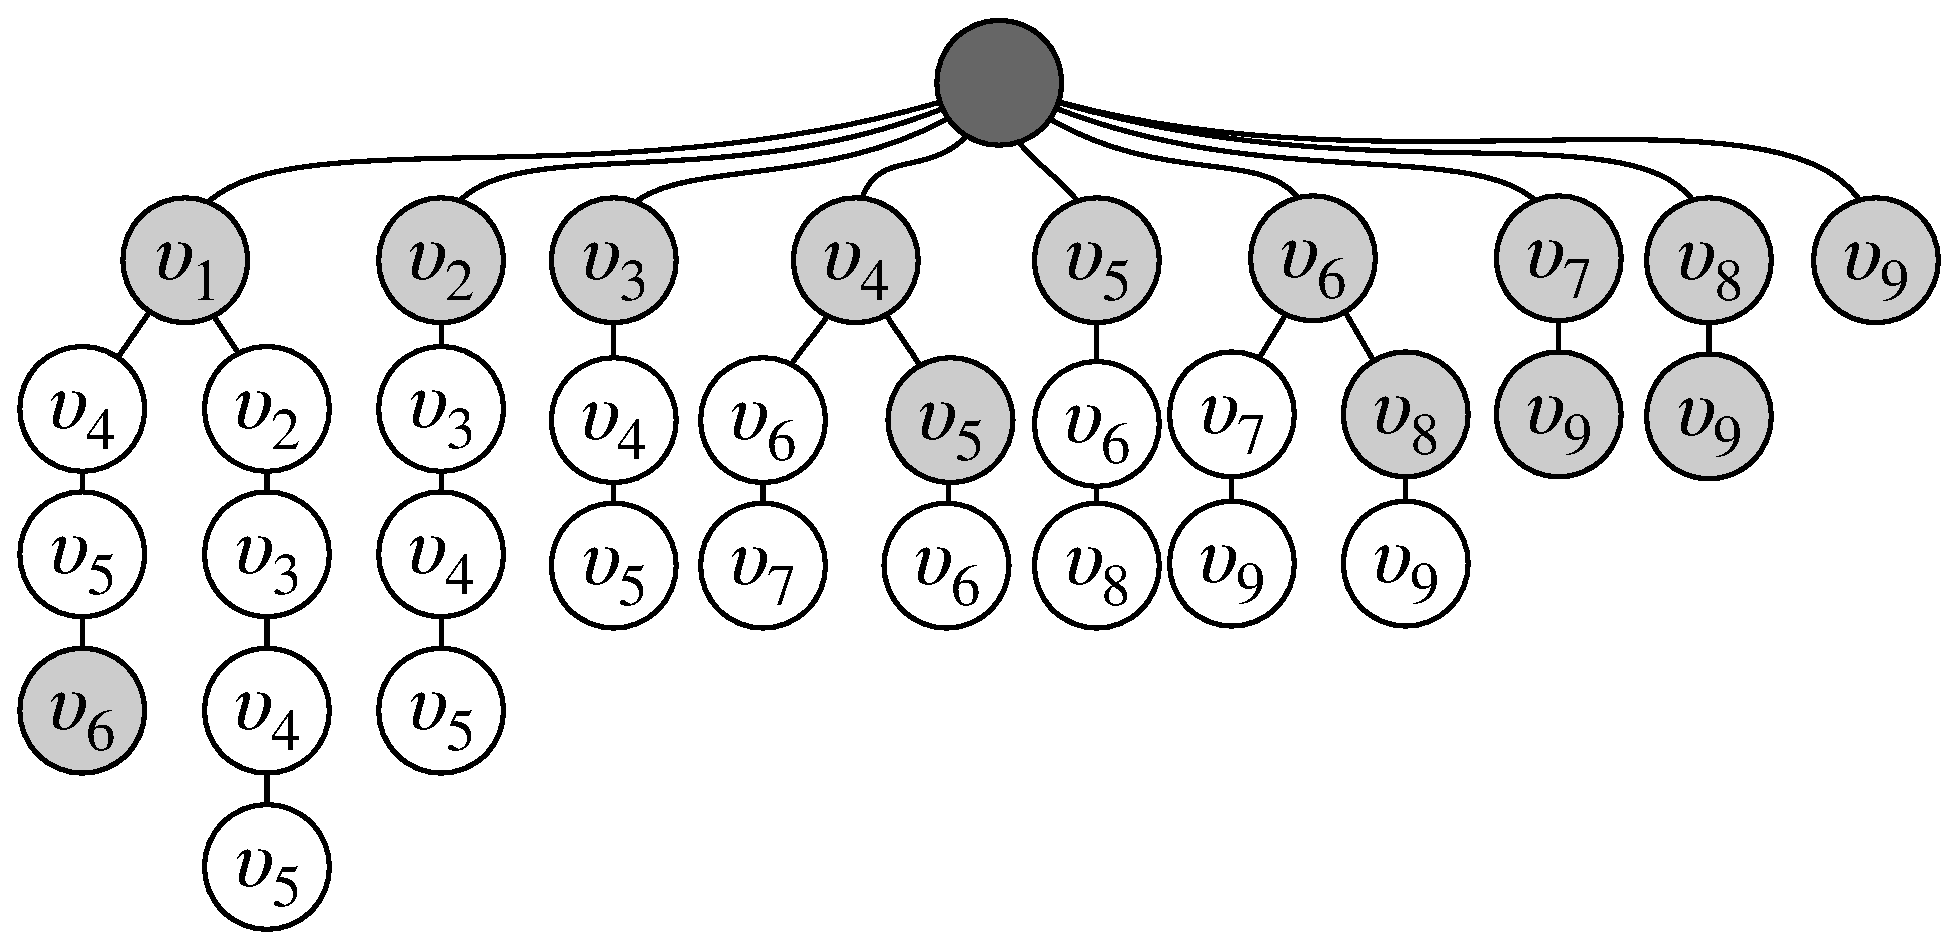
\includegraphics[width=0.9\textwidth]{figure/tree.eps}
%     \caption{An example of a Succinct Clique Tree (SCT). The white nodes represent pivots.}
%     \label{fig:sct_example}
% \end{figure*}
\begin{figure}[tb]
    \centering
    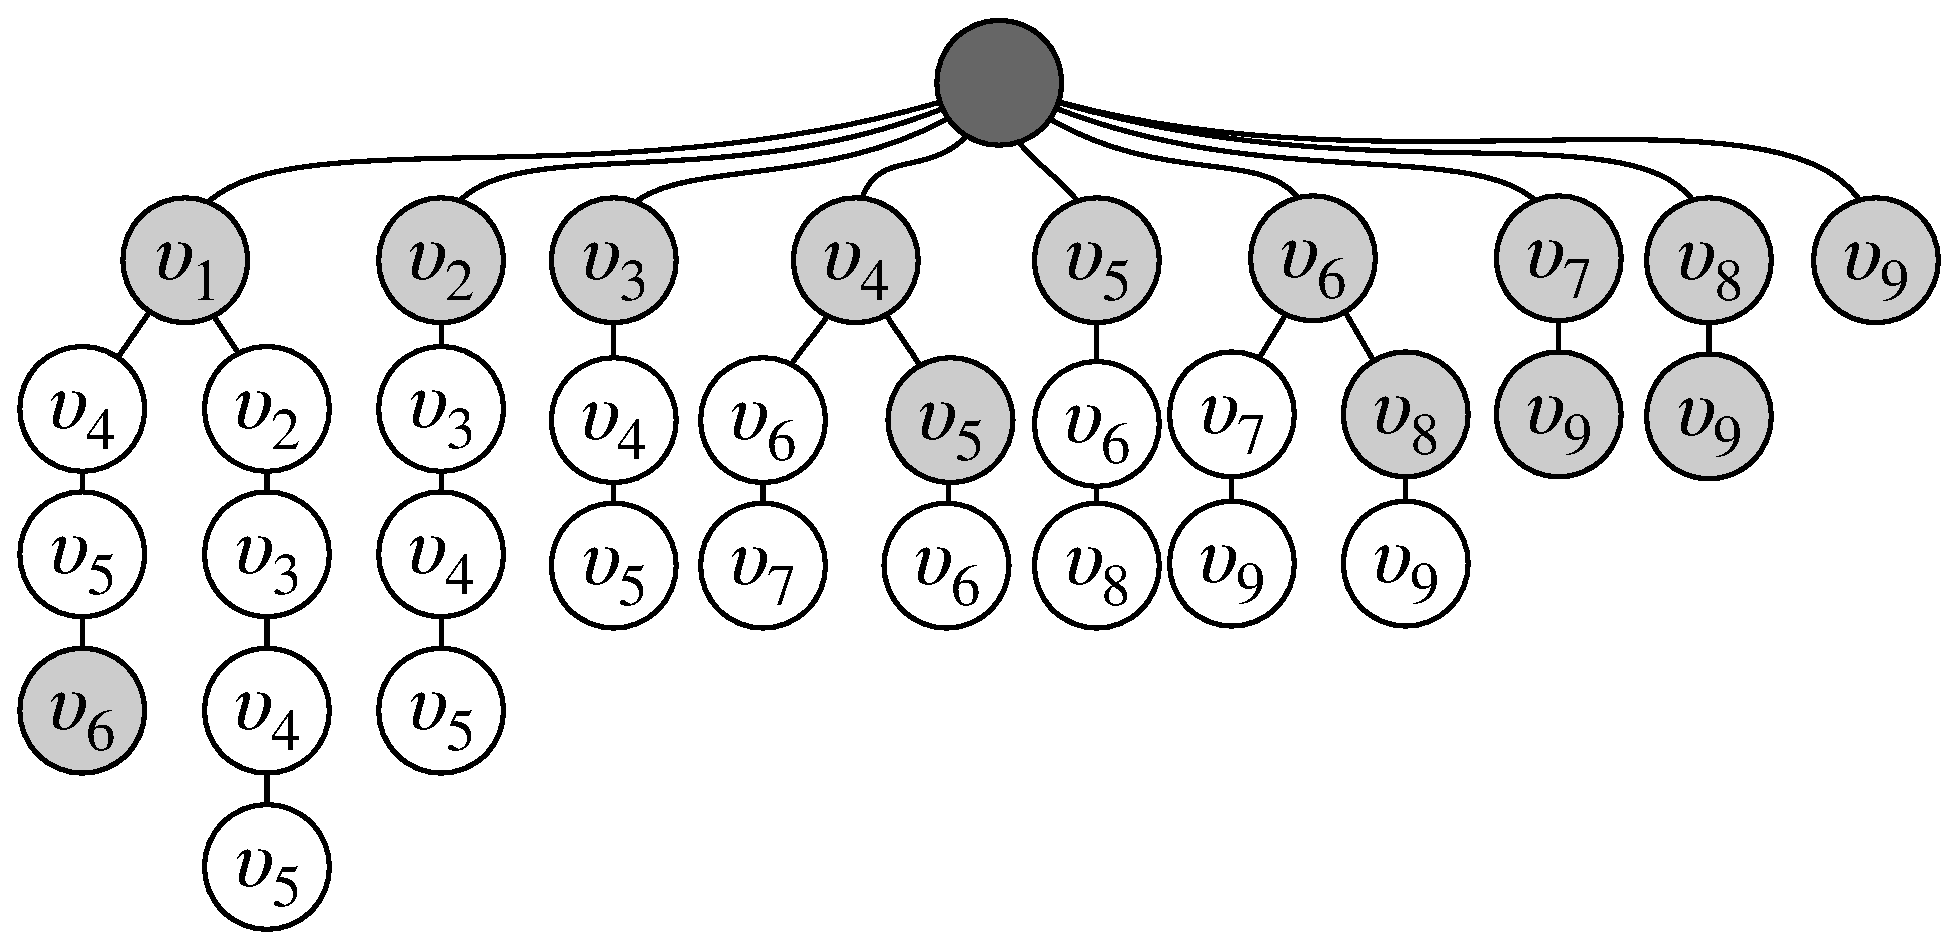
\includegraphics[width=0.43\textwidth]{figure/tree.eps}
    \caption{An example of a Succinct Clique Tree (\sct). White nodes denote pivots; gray nodes denote holds.}
    \label{fig:sct_example}
\end{figure}

% 基于出名的Bron-Kerbosch的理论, \cite{Pivoter}对此进行了一些改进, 提出了一个基于压缩的Succinct Clique Tree (SCT)的表示方法. 他们删除了$X$集合, 只保留$R$和$P$两个集合, 如Algorithm~\ref{alg:buildSCT}所示.
% The Bron--Kerbosch algorithm\cite{BronKerbosch,bitsetClique} is a seminal backtracking scheme for enumerating maximal cliques. Building on the same pivoting-style search space, Pivoter\cite{Pivoter} introduced the Succinct Clique Tree (SCT), which organizes the recursion into a compact multiway structure. Each state carries two sets: a \emph{hold} set $V_h$ (vertices already selected) and a \emph{pivot} set $V_p$ (eligible extensions), compactly capturing families of cliques. Figure~\ref{fig:sct_example} shows the SCT constructed for the example graph in Figure~\ref{fig:graph_example}.

% The Bron-Kerbosch algorithm\cite{BronKerbosch,bitsetClique} is a seminal back-tracking scheme for enumerating all maximal cliques in an undirected graph. 
% Based on the Bron-Kerbosch algorithm, \cite{Pivoter} introduced a Succinct Clique Tree (SCT) representation method that compresses the search space, as shown in Algorithm~\ref{alg:buildSCT}. The algorithm ultimately generates a multi-way tree, where each clique path represents a clique.
Figure~\ref{fig:sct_example} illustrates the SCT constructed for the example graph shown in Figure~\ref{fig:graph_example}.
% 为了方便后续介绍, 我们定义了根到叶子的路径, 如下所示:
We first define a \textit{clique path} as follows: 


\begin{definition}[Clique Path]\label{def:root_leaf_path}
In a Succinct Clique Tree, a \emph{clique path} $\TPath{}$ is any root-to-leaf path.  
All clique paths are enumerated in left-to-right depth-first order, with the $i$-th path denoted by $\TPath{i}$.
Formally,
$
  \TPath{i} = \langle v_{a_1}, v_{a_2}, \dots, v_{a_\ell} \rangle,
$
where $v_{a_1}$ is the root, $v_{a_\ell}$ is the leaf, and $\ell$ is the path length.
\end{definition}


\begin{example}
\label{ex:sct_example}
Figure~\ref{fig:sct_example} shows an example of a \sct. $\TPath{1} = \langle v_1, v_4, v_5, v_6 \rangle$, the second path is
$\TPath{2} = \langle v_1, v_2, v_3, v_4, v_5 \rangle$. There are eleven
clique paths in total, and the last path is $\TPath{11} = \langle v_8, v_9 \rangle$.
\end{example}


% \begin{lemma}[Clique Count in a Path~\cite{Pivoter}]
\begin{lemma}[Unique Path Encoding~\cite{Pivoter}]
\label{lem:clique_count}
% Let $\TPath{}$ be a clique path in an \sct, with
% $V_{p}(\TPath{})$ and $V_{h}(\TPath{})$ denoting its pivot
% and hold vertices, respectively.
% For any $k\ge |V_{h}(\TPath{})|$, every $k$-clique represented by
% $\TPath{}$ consists of all vertices in $V_{h}(\TPath{})$ and
% exactly $k-|V_{h}(\TPath{})|$ vertices chosen from $V_{p}(\TPath{})$.
% Hence $\#\text{$k$-cliques on }\TPath{}$ is equal to $ \binom{|V_{p}(\TPath{})|}{\,k-|V_{h}(\TPath{})|\,}.$

% 对于图中任何的$k$-clique $C_k$, 都存在且仅存在一个根到叶子的路径$\TPath{} = V_h(\TPath{}) \cup V_p(\TPath{})$满足$V_h(\TPath{}) \subseteq C_k \subseteq V_h(\TPath{}) \cup V_p(\TPath{})$. 其中$V_h(\TPath{})$和$V_p(\TPath{})$分别表示路径$\TPath{}$上的hold顶点和pivot顶点集合.
For any $k$-clique $C_k$ in the graph, there exists only one clique path $\TPath{} = V_h(\TPath{}) \cup V_p(\TPath{})$ such that $V_h(\TPath{}) \subseteq C_k \subseteq (V_h(\TPath{}) \cup V_p(\TPath{}))$. Here, $V_h(\TPath{})$ and $V_p(\TPath{})$ denote the sets of hold vertices and pivot vertices on the path $\TPath{}$, respectively.
\end{lemma}

Intuitively, any $k$-clique represented by a path $\TPath$ must include all hold vertices of that path, while the pivot vertices are optional. 
%
Formally, a $k$-clique $C_k$ is \emph{encoded} by a \cpi\ path $\TPath$ if and only if $V_h(\TPath) \subseteq C_k \subseteq V_h(\TPath) \cup V_p(\TPath)$; 
it is \emph{covered} by $\TPath$ if and only if  $C_k \subseteq V_h(\TPath) \cup V_p(\TPath)$.


\begin{example}
  For \sct as shown in Figure~\ref{fig:sct_example}.
  $V_{p}(\TPath{1}) = \{v_4, v_5\}$ and
  $V_{h}(\TPath{1}) = \{v_1,v_6\}$. Thus, the number of $3$-cliques on $\TPath{1}$ is equal to $ \binom{2}{\,3-2\,} = 2.$ $V_{p}(\TPath{2}) = \{v_2, v_3, v_4, v_5\}$ and $V_{h}(\TPath{2}) = \{v_1\}$. Thus, the number of $3$-cliques on $\TPath{2}$ is equal to $ \binom{4}{\,3-1\,} = 6.$
\end{example}

% \noindent\textit{Scope.}

\stitle{Inadequacies in \sct Structures.} 
\sct is designed solely for clique counting on static graphs. 
For the key functions in our framework (Algorithm~\ref{alg:framework}), 
\sct can support \textsc{$s$-CliqueCount} (i.e., initializing the support) with minor modifications. 
However, it lacks dynamic update capabilities and cannot be trivially extended to support \textsc{UpdateIndex} and \textsc{UpdateSupport}, which are required in our representation layer to remove peeled $r$-cliques efficiently. 
%
This limitation motivates the design of a new index that can support all these operations, which is both non-trivial and challenging.


% our Clique Path Index (\cpi) in next subsection, which adapts SCT to support efficient batched updates.
% a static counting structure: it directly supports 
% line~2 (one-shot initialization of $(r,s)$-supports) 
% but does not provide the dynamic path-local updates required by line~9 (removing peeled $r$-cliques from the index) and line~10 (updating neighbors' supports). 
% This limitation motivates our Clique Path Index (\cpi) in next subsection, which adapts SCT to support efficient batched updates.


% (i) \textsc{$s$-CliqueCount}, which initializes the $s$-support for each $r$-clique (Line~2); 
% (ii) \textsc{UpdateIndex}, which removes peeled $r$-cliques (Line~9); and 
% (iii) \textsc{UpdateSupport}, which identifies and updates the supports of affected $r$-cliques after each removal (Line~10). 
